\section{Results}

\subsection{General Results}
After training the models, we evaluated their accuracies on the remaining trading data ranging from 01.11.2019 to 31.12.2019.
Before applying the model on the test data, we excluded bins for which no volume was traded 
in the following bin or lagged values are not available, as was already done to the training set.

\begin{figure}[H]
    \captionsetup{format=plain}
    \makebox[\textwidth]{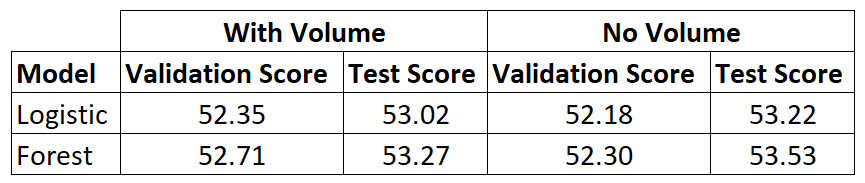
\includegraphics[width=200mm]{all/all_training_results.png} }
    \caption{ 
        This table illustrates the accuracy both for the validation and test set for different feature selection. 
    }
    \label{stats:training_results}
\end{figure}

For the Logistic Regression, we achieved an accuracy of 53.23\% and 53.02\% with and without volume respectively.
The Random Forest achieved an accuracy of 53.54\% and 53.28\% with and without volume respectively (see figure \ref{stats:training_results}).
As one can see for most models, the incorporation of volumes makes no discernable difference.
These accuracies are not out of the ordinary when comparing their performance to the results of other methods (see <cite Predicting price>).
Due to this and reduced amount of computational effort, we decided to continue with models that were trained
without volume.


\begin{figure}[H]
    \captionsetup{format=plain}
    \makebox[\textwidth]{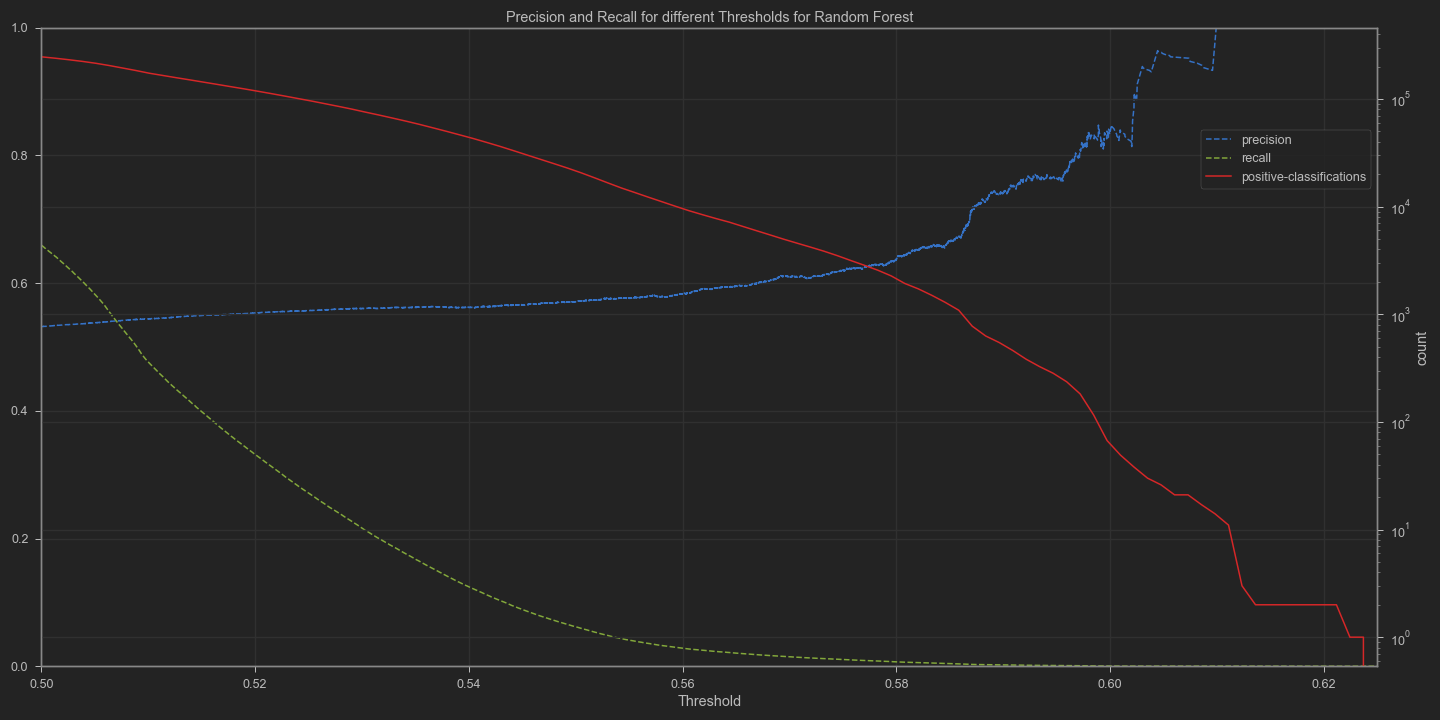
\includegraphics[width=200mm]{forest/rf_precision_vs_threshold.png} }
    \caption{ 
            This figure illustrates the precision, recall and up-classifications of the Random Forest for different thresholds
            without taking volume into consideration. 
        }
    \label{fig:rf_precision_vs_threshold}
\end{figure}


Figure \ref{fig:rf_precision_vs_threshold} illustrates the precision, recall and up-classifications of the Random Forest for different thresholds.
The slope of the precision of remains relatively stable up until a threshold of 0.58 after which a strict increase takes place for increasing thresholds.
On one hand, this comes with the tradeoff that drastically less up-classifications take place, 
which in turn leads to less trades for the trading algorithm, thus less potential return.
On the other hand, strong probability signals indicate relatively high up-movements and low error probabilities, 
thus higher returns per trade and profitability after transaction cost.
Therefore, it is paramount to fine tune the threshold in order to avoid costly missclassification.
Only judging from the aforementioned figure, the highest returns will be achieved somewhere around 
a classification threshold of 0.6, since there are still a considerable amounts of trades in
combination with high precision.
In chapter \ref{ch:strategy_performance}, we demonstrate how changing thresholds leads to drastic
differences in terms of return and profitability.




% \begin{figure}[H]
%     \captionsetup{format=plain}
%     \makebox[\textwidth]{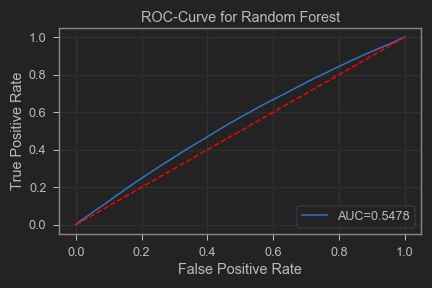
\includegraphics[width=200mm]{rf_roc_curve.png} }
%     \caption{ 
%             This figure illustrates the ROC-curve for the Random Forest without taking volume into consideration. 
%             The predictive performance of the dashed line in terms of ROC would be achieved in theory by assigning class labels completely randomly.
%         }
%     \label{fig:rf_roc_curve}
% \end{figure}


% \begin{figure}[H]
%     \captionsetup{format=plain}
%     \makebox[\textwidth]{\includegraphics[width=200mm]{confusion_matrix_no_volume_logistic_120min.png} }
%     \caption
%         {This plot illustrates the accuracy of Logistic Regression and Random Forest for different feature specifications.
%         Before applying the model on the test data, we excluded bins for which no volume was traded 
%         in the following bin or lagged values are not available, as was already done to the training set.
%         }
%     \label{fig:confusion_matrix_logistic_120min}
% \end{figure}



\subsection{Strategy Performance} \label{ch:strategy_performance}
In this chapter, we outline the performance after employing the trading algorithm on the 
trading set as described in chapter \ref{ch:trading_algorithm}.
Figure \ref{fig:rf_returns_by_thresholds} illustrates total returns using the Random Forest for probability signals when employing the trading 
algorithm for different classification threshold levels. 
For low probability thresholds, the returns are strongly negative, since due to the low precision (see figure \ref{fig:rf_precision_vs_threshold}),
a high amount of missclassifications take place. 
These missclassification then cancel off the positive returns in case of a correct classification.

\begin{figure}[H]
    \captionsetup{format=plain}
    \makebox[\textwidth]{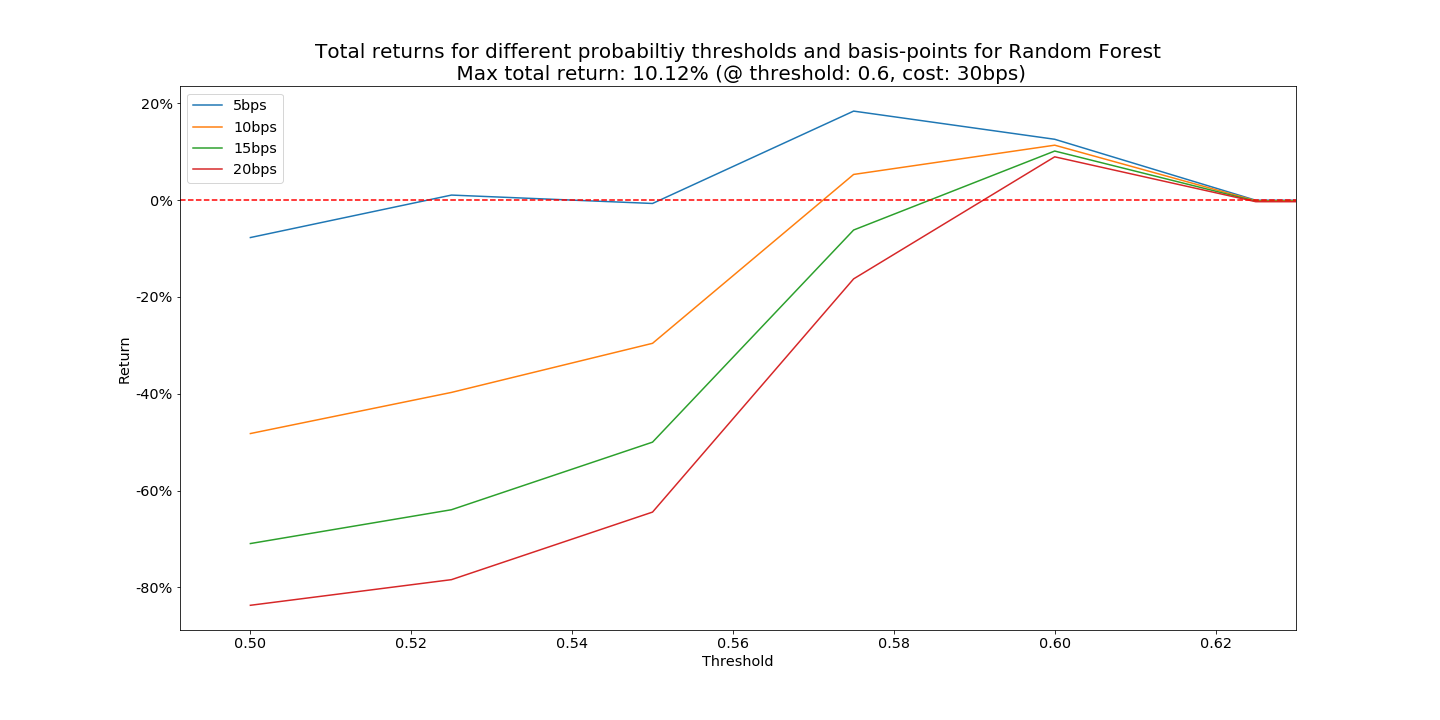
\includegraphics[width=200mm]{forest/rf_total_returns_by_thresholds.png} }
    \caption{ 
            This figure illustrates total returns using the Random Forest for probability signals when employing the trading 
            algorithm for different classification threshold levels. 
            These returns are also further subjected to different levels of transaction cost (10, 20, 30 and 40 bps).
        }
    \label{fig:rf_returns_by_thresholds}
\end{figure}

Further, because a weak probability signal is sufficient to surpass the threshold, 
the proportion of correct classification with insufficient returns is higher, as can be seen in figure \ref{fig:proportion_insufficient_returns}.
Even though the algorithm chose the correct position according to the price movement,
the actual realized return can be below the transaction cost, which causes further decline in total return.
Therefore, increasing the threshold also increases the proportion of classifications with sufficient return,
since these observations with such returns tend to exhibit stronger probabilities.


\begin{figure}[H]
    \captionsetup{format=plain}
    \makebox[\textwidth]{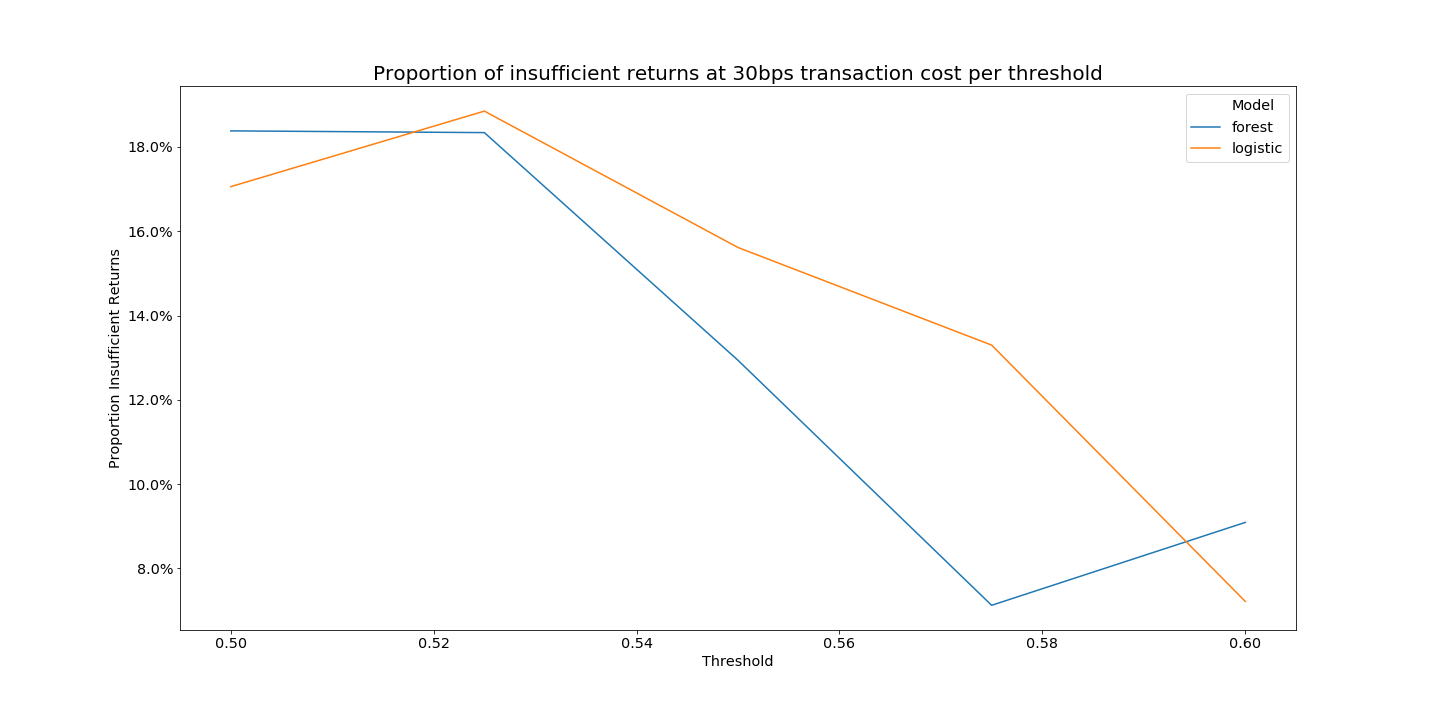
\includegraphics[width=200mm]{all/all_proportion_insufficient_returns.png} }
    \caption{ 
            This figure illustrates the total proportion of correct trading decision according to the price movement with 
            insufficient returns at 30bps transaction cost for different thresholds. 
            These returns are insufficient, because they are below the 30bps which leads to effectively negative returns.
        }
    \label{fig:proportion_insufficient_returns}
\end{figure}

For increasing probability threshold, the returns also tend increase up until 9.87\% at 30bps for the Random Forest, 
which can also be explained with the aforementioned implications 
from figure \ref{fig:rf_precision_vs_threshold} and \ref{fig:rf_returns_by_thresholds}. 
Even when introducing different levels of transaction cost, the returns are consistently positive
for a threshold of 0.6 converging to similar values. 
The convergence can be explained by the fact that considerably less trades take place for high threshold values as can be seen in figure \ref{fig:rf_precision_vs_threshold}.
Since less trades are conducted, the implicit compound interest effect of transaction cost is drastically reduced,
thus slight changes in costs do not affect overall profitability as much. 
Finally, after a certain threshold level, virtually no positive classifications take place according to figure \ref{fig:rf_precision_vs_threshold},
thus leading to zero returns eventually, which can also be seen for the Logistic Regression in figure \ref{fig:logistic_returns_by_thresholds}.

\begin{figure}[H]
    \captionsetup{format=plain}
    \makebox[\textwidth]{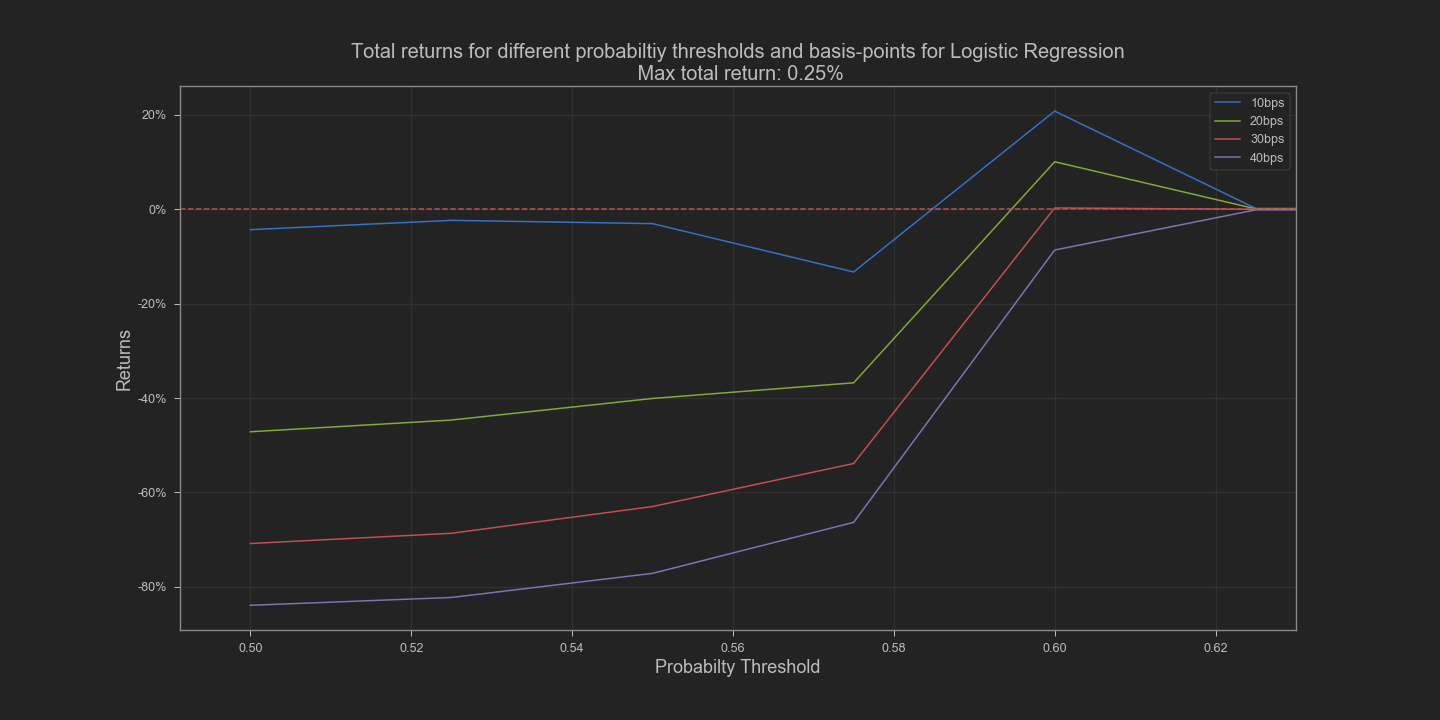
\includegraphics[width=200mm]{logistic/logistic_total_returns_by_thresholds.png} }
    \caption{ 
            This figure illustrates total returns using the Logistic Regression for probability signals when employing the trading 
            algorithm for different classification threshold levels. 
            These returns are also further subjected to different levels of transaction cost (10, 20, 30 and 40 bps).
        }
    \label{fig:logistic_returns_by_thresholds}
\end{figure}




\subsection{Further Analyses}
In this chapter, we analyse how the different return deltas impacted the predictions ofthe model.

Figure \ref{fig:rf_feature_importances} illustrates the feature importances for the Random Forest according to MDI \cite{louppe2015variableImportance}
for different return deltas in minutes (see chapter \ref{ch:feature_and_target}).
Surprisingly, the overall shape of of the graph is concave peaking a 60 min 
instead of peaking right at the beginning and then monotonously decreasing in importance.
As one can see, after a return delta of 10 hours, the relative importance remains low. 
This indicates that returns over a long period of time exhibit a relatively low explanatory power for
predicting price movements.

Figure \ref{fig:logistic_coefficients} illustrates the coefficients for the Logistic Regression 
for different return deltas in minutes. Comparing the absolute coefficient values of with the MDI values 
from the Random Forest, the effect of the return deltas seems to be inverted. 
The highest coefficient values are realized at the beginning and at the end which is
in stark contrast to the Random Forest. However, these findings should be viewed critically, 
since almost all coefficients exhibit insignificant t-statistic values indicated by the blue color.


\begin{figure}[H]
    \captionsetup{format=plain}
    \makebox[\textwidth]{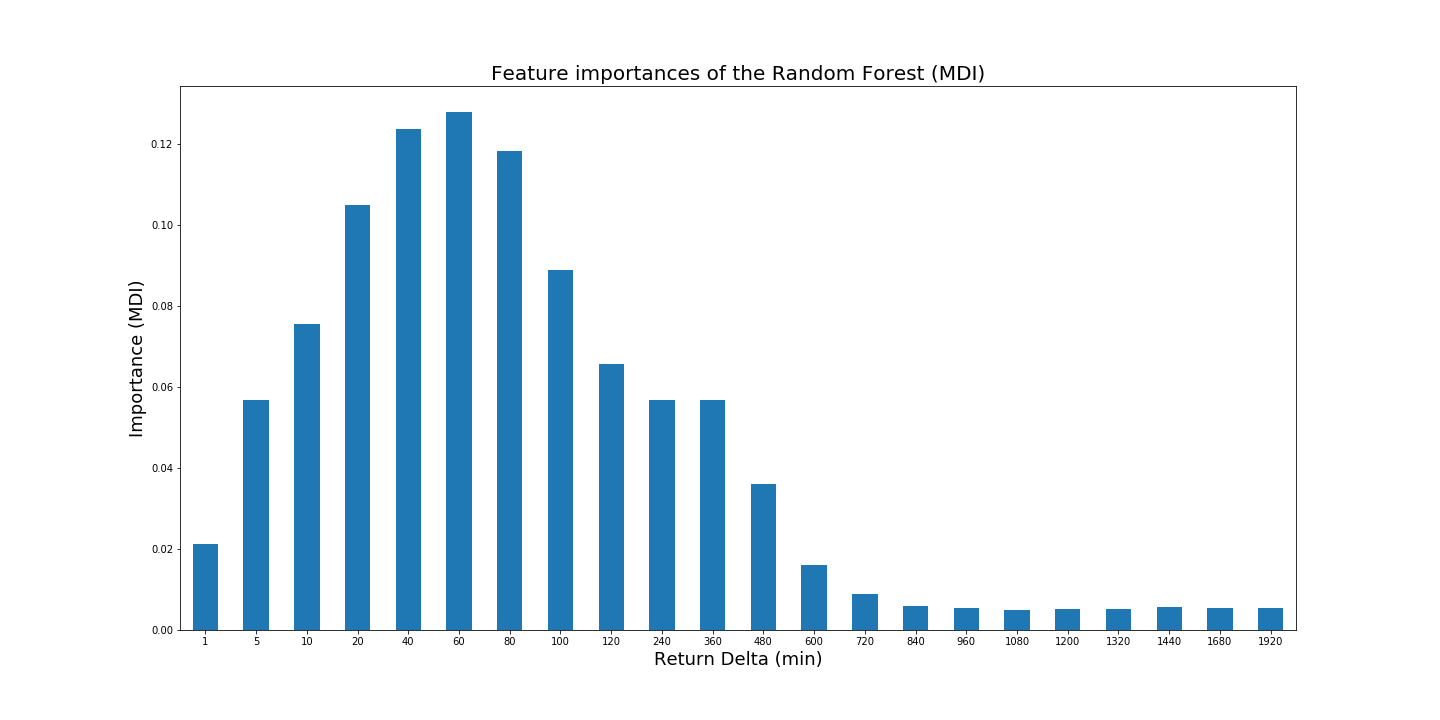
\includegraphics[width=200mm]{forest/rf_feature_importances.png} }
    \caption{ 
            This figure illustrates the feature importances for the Random Forest according to MDI \cite{louppe2015variableImportance}
            for different return deltas in minutes as described in chapter \ref{ch:training_trading}.
        }
    \label{fig:rf_feature_importances}
\end{figure}

\begin{figure}[H]
    \captionsetup{format=plain}
    \makebox[\textwidth]{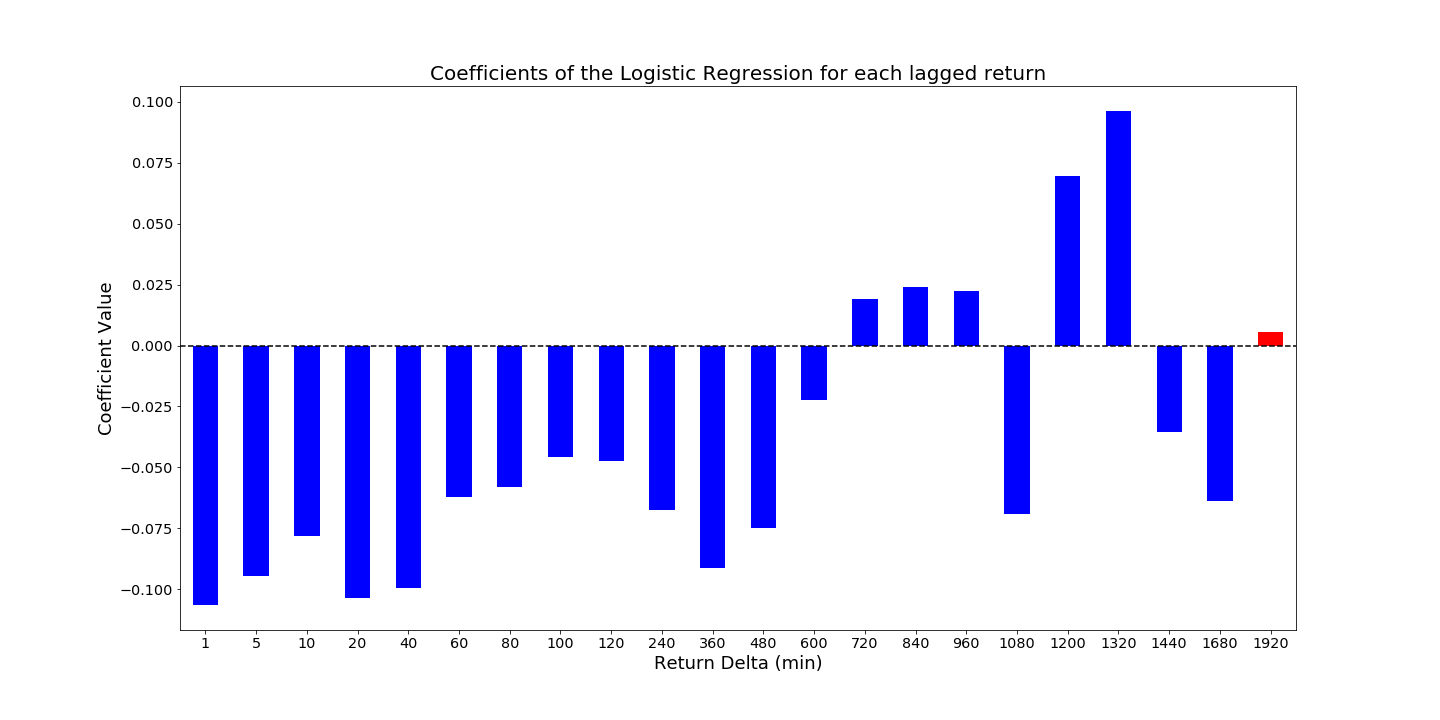
\includegraphics[width=200mm]{logistic/logistic_coefficients.png} }
    \caption{ 
            This figure illustrates the coefficients for the Logistic Regression 
            for different return deltas in minutes as described in chapter \ref{ch:training_trading}.
            The blue bars indicate non-significant coefficient according to the t-test whereas the red ones are
            significant.
        }
    \label{fig:logistic_coefficients}
\end{figure}
